\documentclass[12pt]{article}
% \usepackage[breaklinks=true]{hyperref}
% \usepackage[html,png]{tex4ht}
\usepackage{color}
\usepackage{amsmath,amssymb,amsthm}
\usepackage{natbib}
\usepackage{array}
\usepackage{booktabs, multicol, multirow}
\usepackage[nohead]{geometry}
\usepackage[singlespacing]{setspace}
\usepackage[bottom]{footmisc}
\usepackage{floatrow}
\usepackage{float}
\usepackage{caption}
\usepackage{indentfirst}
\usepackage{lscape}
\usepackage{floatrow}
\usepackage{epsfig}
\usepackage[usenames,dvipsnames,svgnames,table]{xcolor}
\usepackage[colorlinks=true,
            urlcolor=RawSienna,
            linkcolor=RawSienna,
            citecolor=NavyBlue]{hyperref}
\floatsetup[table]{capposition=top}
\floatsetup[figure]{capposition=top}


\newcommand{\beq}{\begin{equation}}
\newcommand{\eeq}{\end{equation}}

\newcommand{\cD}{{\mathcal D}}
\newcommand{\cF}{{\mathcal F}}
\newcommand{\todo}[1]{{\color{red}{TO DO: \sc #1}}}
\renewcommand{\baselinestretch}{1.5}

\title{Student Evaluations of Teaching (Mostly) Do Not Measure Teaching Effectiveness}
\author{Anne Boring, Kellie Ottoboni, Philip B.~Stark}
\date{Draft \today}
\begin{document}
\maketitle

\newpage
\begin{quotation}
    \emph{The truth will set you free, but first it will piss you off.}
    
     \hfill Gloria Steinem

\begin{abstract}

We examine whether student evaluations of teaching (SET) 
primarily measure teaching effectiveness, using nonparametric tests applied
to two datasets. 
For the first dataset, 23,001~SET of 379~instructors by 4,423~students in six 
mandatory first year courses in a five-year natural experiment at a French university, 
we study relationships among SET and the genders of students and instructors, 
grade expectations, and grades.
For the second dataset, 43~SET for 4~sections of an online course in a randomized, controlled, 
blind experiment at a US university, 
we study the relationships among SET, the genders of students, 
the actual and perceived genders of instructors, and grades.
Instructors perceived to be female receive lower SET scores by an amount that is large and
statistically significant.
There are also statistically significant positive associations between SET and expected grades. 
However, SET are not significantly associated with an objective measure of teaching effectiveness,
student performance on anonymously graded finals. 
This suggests that SET do not primarily measure instructors' 
effects on student learning. 
Rather, they primarily measure student biases and expectations.
There is strong statistical evidence that at the aggregate level, relying on SET for 
personnel decisions disadvantages female instructors.
The biases vary by student and by subject, making it 
difficult or impossible to adjust for the bias. 

% Nonparametric permutation tests that aggregate within 1,194 course sections show: 
%\begin{itemize}
%   \item the association between SET and final 
%            exam scores is negative but insignificant
%            ($P \approx 0.70$)
%   \item the association between SET and grade 
%            expectations is positive and highly significant
 %           ($P \approx 0.00$)
%   \item the association between instructor gender 
%            and final exam scores is insignificant
%            (students of male instructors do worse, $P\approx 0.51$ overall, $0.76$ for male students, $0.65$ for female students)
%   \item the association between instructor gender and SET is highly significant---because male
%             students rate male instructors higher 
%            (men get higher ratings, $P \approx 0.00$ overall, $0.00$ for male students,
%            $0.49$ for female students)
%\end{itemize}
%These relationships vary by discipline. 

%all first-year students take the same courses 
%(economics, history, political science, sociology, and %political institutions). 
%Students are assigned to sections of those courses as if %at random, creating a natural experiment.
%Final exams are set for the entire course
%by the professor rather than the section instructor, and %are graded anonymously.
%Hence, final exam scores are a proxy for the %effectiveness of the section instructors.
%SET are mandatory.
%
%Student responses fail simple tests of data quality.
%For instance, 29\% of students report spending impossible amounts of time
%on their courses.

\end{abstract}

\newpage

\end{quotation}

\section{Background}
Student evaluations of teaching (SET) are used widely 
in decisions about hiring, promoting, and firing instructors, especially non-tenured 
higher-education faculty. 
Universities generally treat SET as a measure of teaching effectiveness or teaching quality, 
rather than, e.g., a measure of student satisfaction.
Measuring teaching effectiveness is difficult---for students,
faculty, and administrators alike.
Evaluation surveys may measure something other than teaching effectiveness:
they may be consciously or unconsciously biased. 
In this article, we adopt the definition by \citet[p.17]{Centra2000}, according to whom 
biases in SET occur when ``a teacher
or course characteristic affects teacher evaluations, either positively or
negatively, but is unrelated to criteria of good teaching, such as increased student learning." 

Randomized experiments show that students confuse grades 
(or grade expectations) with long-term value \citep{Carrell2010a,Braga2014}. 
These experiments found that SET scores are not associated with 
student performance in follow-on courses, i.e., with effectiveness. 
Instead, high SET appear---on the whole---to be a reward students give 
instructors who are easy graders or who ``teach to the test.''  

Gender also affects how students rate instructors.
\citet{Boring2015} finds that SET are affected by gender biases and stereotypes. 
Male first-year undergraduate students tend to give more \textit{excellent} scores to male instructors,
even though there is no difference between
the academic performance of students of male and of female instructors.
Recent experimental work by \citet{MacNell2014} finds that
students rate the very same instructor lower on every aspect of teaching,
including ``objective'' measures such as timeliness, when they think the instructor is 
female than when they think the instructor is male. 

Here, we use the datasets of \citet{Boring2015} and \citet{MacNell2014} to investigate 
whether SET scores, including the overall satisfaction score, 
primarily measure teaching effectiveness or something else---biases.
The two main sources of bias we study are students' grade expectations and the gender of the 
instructor. 
We also investigate differences in bias by discipline using data from \citet{Boring2015}.

We use permutation tests that allow us to avoid 
contrived, counterfactual assumptions about
generative models for the data, which regression-based methods (including
ordinary linear regression, mixed effects models, logistic regression, etc.) and parametric
methods such as $t$-tests and ANOVA generally require.
The null hypotheses for our tests are that some 
characteristic---e.g., instructor gender---amounts to an arbitrary label and might as well
have been assigned at random. 

We work with course-level summaries, matching how institutions use SET: 
typically, student responses in a given course
are averaged, and those averages are compared across instances of the course,
across courses in a department, across instructors, and across departments.
Statistical problems with this reduction to and reliance upon averages are 
discussed by \citet{StarkFreishtat2014}.

We find that associations between objective measures of teaching effectiveness and SET are weak
and not statistically significant.
Gender biases are stronger determinants of SET than teaching effectiveness is.
Instructors perceived to be male receive significantly higher SET scores on average:
in the French data, \emph{male} students tend to rate male instructors higher
than they rate female instructors, with no difference in ratings by female students;
in contrast, in the US data, \emph{female} students tend to rate (perceived) male instructors 
higher than they rate (perceived) female instructors, with no difference in ratings by male students. 
The French data also show that gender biases vary by course topic, and 
that students conflate grade expectations with teaching effectiveness.
We therefore conclude that SET primarily do not measure teaching effectiveness; that
they have strong biases unrelated to actual teaching effectiveness; that the biases are not uniform;
and that it is impossible to adjust for these biases. 
The strong gender biases and the weak association between SET and student performance
imply that SET should not be relied upon as a measure of teaching effectiveness.
In particular, reliance on SET for personnel decisions has disparate impact. 

\section{Methods and Notation}
We use the Neyman ``potential outcomes'' framework.
A fixed number $N$ of individuals---typically, students---is randomized (either truly, or
as if by Nature) into 
$k \ge 2$ groups of sizes $N_1, \ldots, N_k$.
Each group receives a different treatment.
``Treatment'' is notional. 
For instance, the treatment might be the gender of the
instructor in the class the student takes.

For each individual $i$, we observe a numerical response $R_i$.
If individual $i$ is assigned to treatment $j$, then $R_i = r_{ij}$.
The numbers $\{r_{ij}\}$ are considered to have been fixed before the experiment.
Implicit in this notation is the \emph{non-interference} assumption that
each individual's response depends only on which treatment that individual receives, 
and not on the treatments other individuals receive.
We observe only one potential outcome for individual $i$, 
depending on which treatment she or he receives.
The responses $\{R_i\}_{i=1}^N$ are random, but only because individuals are 
assigned to treatments at random.

Our approach relies on the distribution induced by the random
assignment, with no assumption about the distribution of SET or other variables, 
no parameter estimates, and no model other than the potential outcomes 
framework with non-interference.

To illustrate the approach in detail, consider the experiment conducted by \citet{MacNell2014},
in which $N$ students were assigned at random to four sections of an online course
in which the students neither saw nor heard the section instructor: interaction was online, with no
audio or video.
Two sections were taught by a female instructor and two by a male instructor.
In one section taught by each instructor, that instructor used a female name; in the other, 
that instructor used a male name.
Students were given comparable biographies for the instructors in all four sections.
Assignments were returned at the same time in all sections.
We observe the SET each student gave the instructor of his or her section;
we do not know what SET the student would have given that instructor had that instructor
used a name with a different gender, nor what SETs the student would have given the other instructor.

In the notation above, each student $i$ could be assigned to any of $k=4$ treatment conditions:
either of two instructors, each identified as either male or female.
Let $r_{i1}$ and $r_{i2}$ be the ratings student $i$ would give instructor A when instructor 
A is identified as male and as female, respectively, and let 
$r_{i3}$ and $r_{i4}$ the ratings student $i$ would give instructor B when that instructor
is identified as male and as female, respectively.
The assignment was made at random: each of the
\beq
 {{N}\choose{N_1 N_2 N_3 N_4}} = \frac{N!}{N_1! N_2! N_3! N_4!}
\eeq
possible assignments of $N_1$ students to instructor A identified as male,
$N_2$ student to instructor A identified as female, etc., was equally likely.

In general, the null hypotheses we test assert that for each $i$, some subset of
$\{r_{ij}\}$ are  equal.
For assessing whether the identified gender of the instructor affects SET,
the null hypothesis is that for each $i$,
$r_{i1} = r_{i2}$ (the rating the $i$th student would give instructor A is the same,
whether instructor A is identified as male or female), 
and $r_{i3} = r_{i4}$ (the rating the $i$th student would give instructor B is
the same, whether instructor B is identified as male or female).
Different students might give different ratings
under the same treatment condition
(the null does not assert that $r_{ij} = r_{\ell j}$ for $i \ne \ell$), and
the $i$th student might 
give different ratings to instructor A and instructor B
(the null does not assert that $r_{i1} = r_{i3}$).
The null hypothesis makes no assertion about the (population) distributions of 
$\{r_{i1}\}$ and $\{r_{i3}\}$.

For student $i$, we observe exactly one of $\{r_{i1}, r_{i2}, r_{i3}, r_{i4}\}$.
If we observe $r_{i1}$, then---if the null hypothesis is true---we also know what $r_{i2}$ is,
and vice versa, but we do not know anything about $r_{i3}$ or $r_{i4}$.
Similarly, if we observe $r_{i3}$ or $r_{i4}$, we know the value of the other, if the
null is true, but we do not know anything about $r_{i1}$ or $r_{i2}$.

Consider the average of the SET for the $N_2 + N_4$ students
assigned to sections taught by an apparently female instructor, minus the 
average of the SET for the $N_1 + N_3$ students
assigned to sections taught by an apparently male instructor; then
take the absolute value of that difference in averages.
This is the test statistic used by \cite{MacNell2014}.
If there were no difference in how students rated instructors based on the perceived
gender of the instructor, we would expect this absolute difference of averages to be close to
zero.\footnote{%
We would expect it to be a least a little different from zero both because of the luck of the draw
in assigning students to sections and because students might rate the two instructors
differently, regardless of the instructor's perceived gender, and the groups are not all the same size.
}
How ``surprising'' is the observed absolute difference in averages?

Consider the
\beq
{{N_1 + N_2} \choose {N_1}} \times {{N_3+N_4} \choose {N_3}}
\eeq
assignments that keep the same $N_1 + N_2$ students in instructor A's
sections (but might change which of those sections a student is in) 
and the same $N_3 + N_4$ students in instructor B's sections.
For each of those assignments, we know what $\{R_i\}_{i=1}^N$ would
have been if the null hypothesis is true, namely, each would be exactly the same
as its observed value, since those
assignments keep students in sections taught by the same instructor.
Hence, we can calculate the value that the test statistic would have had for each
of those assignments.

Because all ${N}\choose{N_1 N_2 N_3 N_4}$ possible assignments of students
to sections are equally likely, these assignments are also equally likely.
The fraction of those assignments that produce a value of the test statistic that
is at least as large (in absolute value) as the observed value of the test statistic
is the $p$-value of the null hypothesis that \todo{fix}.

\todo{conditioning: argument.}

\todo{one more complication: have to assume under the null that the same students
would not have submitted SET, regardless of which section they were in (if assigned to the
same instructor)}



Most of the alternative hypotheses we consider involve
differences in the potential outcomes for some individuals, for various treatments 
(e.g., that SETs differ by instructor gender or by exam grade). 
Because SET are most often reported as class averages or instructor averages, 
we use differences in means between groups and 
correlations between means of SET and other covariates as the test statistics:
we evaluate SET as they typically would be used.


In some cases, we will test a weaker null hypothesis that particular subsets of each individual's
potential responses are equal.


We estimate $p$-values by simulation, but construct exact confidence bounds for the true
$p$-values based on those estimates.
Code for all our analyses is provided at \url{http://www.github.com/????} \todo{Fix!}
The \cite{MacNell2014} data are available online at \todo{Fix!}.
The \cite{Boring2015} data are not public, owing to French restrictions on human subjects data.

The $p$-value of the test is the probability 
of observing a test statistic ``as 
extreme or more extreme'' as the actual observed value of the test statistic,
if the null hypothesis is true.
In principle, this can be calculated exactly by enumerating all possible
assignments of individuals to treatments; but
in practice, complete enumeration may be prohibitively time consuming. 
Instead, we estimate the $p$-value by simulating a large random sample of assignments.  
The uncertainty in the resulting estimate of the $p$-value is accounted for rigorously through
confidence bounds for the $p$-value (found by inverting exact Binomial tests).


\section{Tests of \citet{Boring2015}}
\subsection{The data}

We first study a census of SET from first-year students at a French university.
The data, collected between 2008 and 2013, comprise 23,001 SET from
4,423 students (57\% women) in 1,177
sections, taught by 379 instructors (34\% women). 
\citet{Boring2015} describes the data in detail; key features include:
\begin{itemize}
   \item All first-year students take the same six mandatory courses: 
            History, Macroeconomics, Microeconomics, 
            Political Institutions, Political Science and Sociology.
            Each course has one professor
            who delivers the lectures (to groups of approximately 900 students). 
            All those professors are male.
            Courses have many sections of 10--24 students. 
            Those sections are taught by a variety of instructors, male and female.
            The instructors have considerable pedagogical freedom.
    
   \item Students enroll in ``triads'' of sections of these courses. 
            The enrollment process
            does not allow students to select individual instructors.
            The assignment of students to sections is ``as if'' at random,
            forming a \emph{natural experiment}.
            
   \item Section instructors assign interim grades during the semester.
            Interim grades are known to the students before they submit SET.
            Interim grades hence measure student grade expectations.
            
   \item Final exams are created by the professor, not the instructors.
            All students in a given course take the same final, regardless of which section they
            are enrolled in.
            Final exams are graded anonymously (in every discipline but Political
            Institutions, which we therefor omit from analyses involving final exam scores).
            Performance on the final exam is therefore a measure of the value the
            section instructor adds: students of more effective instructors should do better on
            the final exam, on average.
    
   \item SET are mandatory: the response rates are nearly 100\%.
   
\end{itemize}

SET include closed-ended and open-ended questions, 
but the item that attracts the most attention is the \emph{overall score}, 
which is treated as a summary of the other items.

The SET data include students' individual evaluations of section
instructors in microeconomics, history, political institutions, and 
macroeconomics for the five academic years 2008--2013, and for 
sociology and political science for the three academic years 2010--2013 
(these two subjects were introduced in 2010). 
The SET are anonymous to the instructors, who have access to them only after 
all grades have been officially recorded.  

\begin{table}[htbp]
  \centering
  \footnotesize 
  \caption{Descriptive statistics of sections}
    \begin{tabular}{lccc}
    \toprule 
                        & \# courses & \# instructors  & \% Female instructors  \\
   \midrule
  \textbf{Overall} &  \textbf{1,194} & \textbf{379}  &\textbf{33.8\%} \\
    History    &               230 &      72          &   30.6\% \\
    Political Institutions  &  229 &      65          &   20.0\% \\    
    Microeconomics   &         230 &      96          &   38.5\% \\
    Macroeconomics   &         230 &      93          &   34.4\% \\
    Political Science &       137 &      49          &   32.7\% \\
    Sociology   &              138 &      56          &   46.4\%    \\
    \bottomrule
    \end{tabular}%
 \label{tab:description}%
 
\textit{Data for one section of Political Institutions were excluded because that 
section had an experimental online format. 
Political Science and Sociology originally were not included in the triad system; instead, students were randomly assigned by the administration to different sections.
} 

\end{table}%
\normalsize

Overall, 34\% of the 1,194 instruction sections were taught by women 
(Table~\ref{tab:description}), but the percentage varies by discipline. 
Only 20\% of Political Institutions sections were taught by women. 
Sociology is almost equally divided between male and female instructors (46.4\% were taught by women). 
Microeconomics and Macroeconomics have more instructors in all, because of higher turnover.

\subsection{Methods}\label{boring:methods}
In this section, we report tests of the relationships among the French data,
on SET, teaching effectiveness, and student behavior.
Our tests aggregate data within course sections, to match how SET are typically
used in personnel decisions. 
Our tests are based on the Neyman ``potential outcomes'' framework for causal inference.
 
Since students sign up for courses in triads without knowing who their instructors will be, 
it seems reasonable to model the assignment of instructors to students as random.
Because there may be cohort and social effects among students in sections (a form of
``interference,'' as the term is used in causal inference), the randomization we
use as the basis of our tests keeps intact the group of students who take each section;
the randomization assigns those (fixed) groups of students at random to instructors.
Equivalently, the randomization assigns instructors at random to sections of the class,
holding the set of students enrolled in each section fixed.
We use the Spearman correlation as the test statistic.  \\

We first test whether SET are a measure of teaching effectiveness intrinsic to an instructor.  
If so, an instructor's ratings should not depend on the group of students she or he teaches.
To check, we model 
Each instructor has a set of potential responses each time s/he teaches, depending on which 
section of students is assigned to the instructor that time.
Under the null hypothesis, each instructor's potential responses are all equal;
different instructors may have different potential responses.

Then we can test whether this is correlated with grades in the class.  
If SET is a measure of teaching effectiveness, then the average grade in courses taught by 
instructors with high SET should tend to be high.  
The tests we run under this framework include the correlation between average SET and average final grade (Table~\ref{tab:finalexam}), average SET and average interim grade 
(Table~\ref{tab:instructor gender}), and average final grade and instructor gender (Table~\ref{tab:genderfinal}).  We perform these tests for all instructors in the data, assuming that they are exchangeable between departments, and also by department, allowing for the possibility that relationships between the variables of interest may vary by discipline. \\

The second sort of analysis aims to test whether students use SET as a reliable or meaningful metric when they rate instructors.  We can think of each course as an experimental unit.  
Each course has an average SET and average grade, and then courses get randomly assigned an instructor.  
A course is represented by a ticket with a number for each instructor, and each number is either the class's average SET or average grade with that instructor.  
Under the sharp null, each course's average SET and average grades will be the same for all instructors.  
Then we can test whether this is average SET is correlated with properties of the instructor (e.g. gender, Table~\ref{tab:instructorgender}).  
Stratifying by gender accounts for intrinsic differences between male and female students.  
It also allows us to identify interactions between student and instructor gender: if relationships between instructor gender and another outcome vary according to student gender, then there is an interaction.  
Here, we continue to aggregate student outcomes within courses, but now we take averages separately for the male and female students.  
These tests include the correlation between SET and gender concordance (Table~\ref{tab:genderconcordance}) and the correlation between final exam grade and gender concordance (Table~\ref{tab:finalconcordance}).

These two approaches, treating the instructors as units versus treating the courses as units, are conceptually different experimental designs.  However, they lead to the same permutation algorithm.


\subsection{Analysis of SET and grades}

Teaching effectiveness is multidimensional (e.g. \citet{Marsh1997}) and is therefore difficult to measure. But effective teaching should generate student learning, suggesting that effective instructors should lead their students to understand and learn more course material. Effective instructors should therefore cause their students to obtain higher grades on the final exams, on average. 

We first test whether SET scores are correlated with higher grades on the final exam, on average by instruction section (Table \ref{tab:finalexam}). The results suggest that SET scores do not always measure actual teaching effectiveness. Overall, final exam grades are not statistically correlated with SET scores (one-sided $p$-value 0.70). The only two courses for which they are correlated are microeconomics and macroeconomics ($p$-values of 0.03 and 0.04). SET scores are uncorrelated with student achievement in the three other courses that are graded anonymously, i.e. history ($p$-value 0.31), political science ($p$-value 0.53) and sociology ($p$-value 0.27). 

\begin{table}[htbp]
  \centering
  \footnotesize 
  \caption{Correlation between average SET scores and final exam grades, by instruction section}
    \begin{tabular}{lcc}
    \toprule 
                        & $\rho$  & $p$-value  \\
   \midrule
    Overall &            -0.02 &       0.70  \\
    History &             0.03 &       0.31  \\
    Macroeconomics &      0.12 &       0.04  \\
    Microeconomics &      0.13 &       0.03  \\
    Political science &  -0.01 &       0.53  \\
    Sociology &           0.05 &       0.27  \\
    \bottomrule
    \end{tabular}%
 \label{tab:finalexam}%
 
  \textit{Note: one-sided $p$-values are reported, since we expect that higher SET scores are likely to be correlated with higher final exam grades.}
\end{table}%
\normalsize




\subsection{The correlation between SET scores and gender}


Although mostly uncorrelated with students' performance on the final exam, SET appear to be much better predictors of gender. Overall, average SET scores and instructor gender are correlated, with male instructors obtaining significantly higher SET scores overall ($p$-value 0.00). There are, however, strong variations by course type (Table \ref{tab:instructorgender}). Male instructors of history, macroeconomics and political institutions courses receive (weakly) significantly higher overall satisfaction scores ($p$-values of 0.07, 0.08 and 0.10 respectively). The relationship is also positive between SET scores and instructor gender for microeconomics, political science and sociology courses, although not significant ($p$-values of 0.58, 0.43 and 0.26 respectively).   

\begin{table}[htbp]
  \centering
  \footnotesize 
  \caption{Analyzing the correlation between average SET score and instructor gender, by course}
    \begin{tabular}{lcc}
    \toprule 
                          & $\rho$  & $p$-value     \\
   \midrule
    Overall &                 0.10       & 0.00     \\
    History &                 0.12       & 0.07     \\
    Political institutions &  0.11       & 0.10     \\
    Macroeconomics &          0.11       & 0.08     \\
    Microeconomics &          0.04       & 0.58     \\
    Political sciences &      0.07       & 0.43     \\
    Sociology &               0.10       & 0.26     \\
    \bottomrule
    \end{tabular}%
 \label{tab:instructorgender}%
  
  \textit{Note: two-sided $p$-values are reported.}
\end{table}%
\normalsize


Do men receive higher SET scores overall because they are better instructors? 
If men were indeed better instructors, then their students should perform better on final exams, on average,
in comparable courses. 
This is not what we find (Table \ref{tab:genderfinal}). 
Indeed, the correlation between student performance and instructor gender is negative, although statistically insignificant ($p$-value 0.51 overall), suggesting that male instructors are not more effective
than female instructors, and perhaps are less effective. 


\begin{table}[htbp]
  \centering
  \footnotesize 
  \caption{Correlation between final exam average and instructor gender, by course}
    \begin{tabular}{lcc}
    \toprule 
                     & $\rho$  & $p$-value    \\
   \midrule
    Overall &            -0.02       & 0.51      \\
    History &            -0.06       & 0.39      \\
    Macroeconomics &      0.00       & 0.97      \\
    Microeconomics &     -0.03       & 0.63      \\
    Political sciences &  0.02       & 0.79      \\
    Sociology &          -0.00       & 0.97      \\
    \bottomrule
    \end{tabular}%
 \label{tab:genderfinal}%
 
  \textit{Note: two-sided $p$-values are reported.}
\end{table}%
\normalsize



So why do male instructors receive higher SET scores? 
SET scores and instructor gender are correlated, because male students tend to give higher SET scores to male instructors (Table \ref{tab:genderconcordance}). 
Our permutation tests confirm the results found by \citet{Boring2015}. 
Gender concordance is a statistically strong predictor of SET scores for men ($p$-value 0.00 overall). 
Male students give higher SET scores to male instructors in all fields. 
The correlations are statistically significant at level 0.1 in history ($p$-value 0.00), macroeconomics ($p$-value 0.04), political science ($p$-value 0.06), political institutions ($p$-value 0.07) and 
microeconomics ($p$-value 0.10). 
The correlation is positive but not statistically significant in sociology ($p$-value 0.15). 

Although gender concordance is correlated with overall satisfaction scores for male students, SET scores of female students are not statistically correlated with instructor gender ($p$-value 0.49 overall). The correlation is negative in some fields (history, political institutions, macroeconomics and sociology) and positive in others (microeconomics and political science), but always statistically insignificant ($p$-values between 0.19 and 0.97).



\begin{table}[htbp]
  \centering
  \footnotesize 
  \caption{Correlation between SET scores and gender concordance}
    \begin{tabular}{lccccc}
    \toprule 
          & \multicolumn{2}{c}{Male student}  &  & \multicolumn{2}{c}{Female student} \\
      & $\rho$  &  $p$-value &  & $\rho$  &  $p$-value    \\
   \midrule
      \quad  Overall &                 0.15       & 0.00 & &  0.02       & 0.49      \\
      \quad  History &                 0.18       & 0.00 & & -0.04       & 0.54      \\
      \quad  Political institutions &  0.12       & 0.07 & & -0.09       & 0.19       \\
      \quad  Macroeconomics &          0.14       & 0.04 & & -0.08       & 0.21     \\
      \quad  Microeconomics &          0.11       & 0.10 & &  0.03       & 0.67       \\
      \quad  Political sciences &      0.16       & 0.06 & &  0.00       & 0.97      \\
      \quad  Sociology &               0.12       & 0.15 & & -0.05       & 0.53      \\
    \bottomrule
    \end{tabular}%
 \label{tab:genderconcordance}%
  
  \textit{Note: two-sided $p$-values are reported.}
\end{table}%
\normalsize




Do male instructors receive higher SET scores from male students because their teaching styles match male students' learning styles? If that were the case, then male students who had male instructors should perform better on the final exam. However, this is not what we find (Table \ref{tab:finalconcordance}). If anything, male students who had male instructors appear to perform worse overall on the final exam (the correlation is negative but statistically insignificant, with a $p$-value 0.76). In history, the negative correlation (-0.11) is weakly statistically significant ($p$-value 0.10). In history, male students therefore give significantly higher SET scores, despite the fact that they appear to learn more from female instructors. These results further suggest that students are not measuring actual teaching effectiveness when they complete their SET. 




\begin{table}[htbp]
  \centering
  \footnotesize 
  \caption{Student performance and gender concordance}
    \begin{tabular}{lccccc}
    \toprule 
          & \multicolumn{2}{c}{Male student}  &  & \multicolumn{2}{c}{Female student} \\
      & $\rho$  &  $p$-value &  & $\rho$  &  $p$-value    \\
                             \midrule
      \quad  Overall &                 -0.01       & 0.76 & &  0.01       & 0.65  \\
      \quad  History &                 -0.11       & 0.10 & &  0.01       & 0.86   \\
      \quad  Macroeconomics &           0.02       & 0.76 & & -0.00       & 0.97   \\
      \quad  Microeconomics &          -0.04       & 0.60 & &  0.00       & 0.94  \\
      \quad  Political sciences &       0.10       & 0.25 & &  0.03       & 0.76  \\
      \quad  Sociology &                0.02       & 0.85 & & -0.01       & 0.94  \\
    \bottomrule
    \end{tabular}%
 \label{tab:finalconcordance}%
  
  \textit{Note: two-sided $p$-values are reported.}
\end{table}%
\normalsize





\subsection{The correlation between SET scores and grade expectations}

Not only are SET scores correlated with gender, but they are also positively and significantly correlated with expected grades (Table \ref{tab:instructor gender}). Political institutions is the only course for which the correlation between expected grades and SET scores is not significant ($p$-value 0.19). The $p$-values in all other courses are close to 0. The correlation coefficients are especially high in history (0.32) and sociology (0.27). They are also high in macroeconomics (0.22), microeconomics (0.19) and political sciences (0.16).



\begin{table}[htbp]
  \centering
  \footnotesize 
  \caption{Analyzing the correlation between average evaluation score and interim grades, by course number}
    \begin{tabular}{lcc}
    \toprule 
                          & $\rho$  & $p$-value  \\
   \midrule
    Overall &                 0.10       & 0.00   \\
    History &                 0.32       & 0.00   \\
    Political institutions &  0.06       & 0.19     \\
    Macroeconomics &          0.22       & 0.00    \\
    Microeconomics &          0.19       & 0.00     \\
    Political sciences &      0.16       & 0.03     \\
    Sociology &               0.27       & 0.00     \\
    \bottomrule
    \end{tabular}%
 \label{tab:instructor gender}%
  
  \textit{Note: one-sided $p$-values are reported.}
\end{table}%
\normalsize




To summarize our results, the fact that SET scores are largely uncorrelated with student achievement measured by students' final exam grades suggests that (male) students may be expressing a gender bias in favor of men when rating instructors. Furthermore, students appear to reward instructors who give them higher interim grades. We conclude that gender and expected grades create biases in SET scores, which are unrelated to effective teaching. 

\section{Tests of \citet{MacNell2014}}

While our analysis of the data in the previous section suggests that SET scores are largely unrelated to teaching effectiveness, the natural experimental setting of the French university data does not enable us to control for potential differences in teaching styles of men and women. We know of two experiments which were able to control for teaching styles: \citet{Arbuckle2003} and \citet{MacNell2014}. These two experiments tend to confirm that students express gender biases in SET scores, rather than reward a teaching style that matches their learning style. In both experiments, students tend to give higher SET scores when they think that the course is being taught by a man, regardless of whether the course is actually taught by a man or a woman. Hence, differences in teaching or learning styles do not seem to explain the differences in men and women's SET scores.

In the \citet{Arbuckle2003} experiment, a group of 352 students watched \textquotedblleft slides of an age- and gender-neutral stick figure and listened to a neutral voice presenting a lecture and then evaluated it on teacher evaluation forms that indicated 1 of 4 different age and gender conditions (male, female, \textquotedblleft old," and \textquotedblleft young")" [\citealp{Arbuckle2003}, p.507]. 
The goal of the experiment was to measure whether \textquotedblleft students' perceptions of a professor's age and gender influence their perceptions of the professor's warmth and enthusiasm". Differences in evaluations could thus only be caused by students' subjective age and gender-biased judgments in evaluating the lecturer's competence. The researchers find that students rated the young male instructors higher than the other three combinations, especially on \textquotedblleft enthusiasm", \textquotedblleft showed interest in subject"  and \textquotedblleft using a meaningful voice tone". 

The results of \citet{Arbuckle2003} are reinforced by those of \citet{MacNell2014} who use a different set-up to control for differences in teaching styles. In their experiment, \citet{MacNell2014} used SET data collected from an online course in which 43 students were randomly assigned to four discussion groups for a course, each taught by one of two assistant instructors (one man and one woman). The two instructors each taught one course under their real identity, while they taught the other course under the other instructor's identity. In this set-up, one group of twelve students thought they had a female instructor when the instructor was actually male, and twelve other students thought they had the male instructor when the instructor was actually female. The two instructors worked together with the main professor of the course, to make sure that they gave similar types of feedback to students, graded papers in exactly the same time frame, etc., so as to limit differences in teaching styles or grading to a strict minimum. 

With this framework, potential gender biases can be tested by controlling for teaching styles. Biases in student ratings can be found by comparing how students rate their instructors as a function of the \textit{actual} versus \textit{perceived} gender of the instructor. \citet{MacNell2014} find that ``the male identity received significantly higher scores on professionalism, promptness, fairness, respectfulness, enthusiasm, giving praise, and the
student ratings index... [...] Students in the two groups that perceived their assistant
instructor to be male rated their instructor significantly higher than did the students in the
two groups that perceived their assistant instructor to be female, regardless of the actual gender
of the assistant instructor." 


\subsection{Methods}\label{macnell:methods}
In this section, we once again use permutation tests, this time to analyze the data provided by \citet{MacNell2014}. The use of permutation tests is especially appropriate in this case, given the small sample of twenty male and twenty-three female students.

Each student's potential responses are represented by numbers on a ticket:
\begin{itemize}
\item the rating that the student would assign to instructor A if instructor A is identified as male
\item the rating that the student would assign to instructor A if instructor A is identified as female
\item the rating that the student would assign to instructor B if instructor B is identified as male
\item the rating that the student would assign to instructor B if instructor B is identified as female
\end{itemize}

Nonresponse: there were 3 nonresponders in group 5 and one in group 6.


The null hypothesis is that the first two numbers are equal and the second two numbers are equal, but the first two numbers might be different from the second two numbers. This corresponds to the hypothesis that students assigned to a given instructor would rate him or her the same, whether that instructor seemed to be male or female. For all students assigned to instructor 1, we know both of the first two numbers if the null hypothesis is true, but we know neither of the second two numbers. Similarly, if the null hypothesis is true, we know both of the second two numbers for all students assigned to instructor 2, but we know neither of the first two numbers for those students. \\

Because of how the randomization was performed, all allocations of students to class sections that preserve the number of students in each section are equally likely.  In particular, all allocations that keep the same students assigned to each actual instructor the same are equally likely.  \\

To test the difference in SET between male-identified and female-identified instructors, we use the difference in means between the two groups as our test statistics (Table~\ref{tab:macnell1}).  We look at the instructors' overall rating as well as their rating in each category.  To approximate the null distributions, we permute students who were assigned to instructor 1 and instructor 2 separately, then allocate students within those two groups to the male-identified and female-identified sections.  This stratified permutation method corresponds to testing the null described above. \\

Additionally, we test the correlation between ratings and the concordance of student and reported instructor gender (Table~\ref{tab:macnell2}), correlation between ratings and concordance of student and actual instructor gender (Table~\ref{tab:macnell3}), and correlation between student grades and actual instructor gender(Table~\ref{tab:macnell4}).  For these tests, we use the Spearman correlation.  The tests involving reported instructor gender use the stratified permutations described above, where as the tests of actual instructor gender simply permute all students irrespective of their instructor's reported gender.

\subsection{Analysis of SET and gender}
We first analyze the correlation between student ratings and the reported instructor gender (Table \ref{tab:macnell1}). A positive result signifies that the perceived male instructor received higher evaluations. We find a weak positive correlation between the perceived gender and overall satisfaction ($p$-value 0.10). The statistical significance is stronger for several of the criteria which students rated: fairness ($p$-value 0.00), giving praise ($p$-value 0.01), caring and promptness (both criteria have $p$-values of 0.04), enthusiasm ($p$-value 0.05), communication ($p$-value 0.06), professionalism and respect (both criteria have $p$-values of 0.07), and being consistent and helpful (both criteria have $p$-values of 0.09). The criteria that were not statistically significant were feedback, responsiveness, being knowledgeable and clear. Our permutation tests confirm and extend the results found by \citet{MacNell2014}.


\begin{table}[htbp]
  \centering
  \footnotesize 
  \caption{Analyzing the difference in mean ratings and reported instructor gender (male minus female)}
    \begin{tabular}{lcc}
    \toprule 
                          & difference in means  & $p$-value  \\
   \midrule
    Overall &                 0.47       & 0.15   \\
    Professional &            0.61       & 0.06   \\
    Respectful			   &  0.61       & 0.06   \\
    Caring &                  0.52       & 0.12    \\
    Enthusiastic   &          0.57       & 0.08     \\
    Communicate        &      0.57       & 0.09     \\
    Helpful   &               0.46       & 0.19     \\
    Feedback   &              0.47       & 0.19     \\
    Prompt    &               0.80       & 0.02     \\
    Consistent   &            0.46       & 0.24     \\
    Fair   &                  0.76       & 0.01     \\
    Responsive   &            0.22       & 0.54     \\
    Praise   &                0.67       & 0.02     \\
    Knowledge   &             0.35       & 0.29     \\
    Clear   &                 0.41       & 0.34     \\
    \bottomrule
    \end{tabular}%
 \label{tab:macnell1}%
  
  \textit{Note: two-sided $p$-values are reported.}
\end{table}%
\normalsize


We then analyze in more detail whether male or female students rated the instructors differently according to perceived gender. While in the previous section we found that male students rated male instructors higher, we find in the \citet{MacNell2014} experiment that the perceived male instructor received significantly higher evaluation scores because female students rated the perceived female instructor significantly lower (Table  \ref{tab:macnell2}). Male students rated the perceived male instructor significantly (though weakly) higher on only one criteria: being fair ($p$-value 0.08). Female students, however, rated the perceived female instructor lower in terms of overall satisfaction ($p$-values of 0.08), along most teaching dimensions: giving praise ($p$-value 0.01), enthusiasm ($p$-value 0.03), caring and fairness ($p$-values of 0.04), being respectful and communication ($p$-values of 0.08), professionalism ($p$-value 0.09) and feedback ($p$-value 0.10). Although the results show a negative correlation between being a (perceived) female instructor and ratings on being helpful, promptness, consistency, responsiveness, knowledge and clarity, the results are not statistically significant.



\begin{table}[htbp]
  \centering
  \footnotesize 
  \caption{Analyzing the correlation between ratings and reported instructor gender, by gender concordance}
    \begin{tabular}{lccccc}
    \toprule 
          & \multicolumn{2}{c}{Both male}  &  & \multicolumn{2}{c}{Both female} \\
                          & $\rho$  &  $p$-value &  & $\rho$  & $p$-value    \\
                          
   \midrule
    Overall &                0.09       & 0.81 & & -0.36    & 0.11   \\
    Professional &           0.22       & 0.52 & & -0.36    & 0.10   \\
    Respectful			   & 0.22       & 0.34 & & -0.36    & 0.10   \\
    Caring &                 0.02       & 1.00 & & -0.46    & 0.05  \\
    Enthusiastic   &         0.09       & 0.82 & & -0.44    & 0.05   \\
    Communicate        &     0.12       & 0.68 & & -0.39    & 0.10  \\
    Helpful   &              0.21       & 0.41 & & -0.24    & 0.35   \\
    Feedback   &             0.04       & 0.90 & & -0.37    & 0.10   \\
    Prompt    &              0.38       & 0.15 & & -0.37    & 0.13   \\
    Consistent   &           0.07       & 0.85 & & -0.34    & 0.18   \\
    Fair   &                 0.41       & 0.09 & & -0.43    & 0.04  \\
    Responsive   &           0.18       & 0.53 & & -0.03    & 0.99  \\
    Praise    &              0.29       & 0.27 & & -0.47    & 0.01  \\
    Knowledge   &            0.08       & 0.78 & & -0.29    & 0.21  \\
    Clear   &                0.06       & 0.76 & & -0.25    & 0.29  \\
    \bottomrule
    \end{tabular}%
 \label{tab:macnell2}%

  \textit{Note: two-sided $p$-values are reported.}
\end{table}%
\normalsize


\begin{table}[htbp]
  \centering
  \footnotesize 
  \caption{Analyzing the correlation between ratings and actual instructor gender, by gender concordance}
    \begin{tabular}{lccccc}
    \toprule 
          & \multicolumn{2}{c}{Both male}  &  & \multicolumn{2}{c}{Both female} \\
                          & $\rho$  &  $p$-value &  & $\rho$  &  $p$-value    \\
                          
   \midrule
    Overall &                -0.07       & 0.72 & &  0.13    & 0.56   \\
    Professional &            0.08       & 0.74 & &  0.04    & 0.95   \\
    Respectful		       &  0.08       & 0.84 & &  0.04    & 0.94   \\
    Caring &                 -0.11       & 0.59 & &  0.03    & 0.98  \\
    Enthusiastic   &         -0.07       & 0.82 & &  0.20    & 0.40   \\
    Communicate        &     -0.01       & 0.84 & &  0.08    & 0.67  \\
    Helpful   &               0.01       & 0.96 & & -0.12    & 0.70   \\
    Feedback   &             -0.12       & 0.69 & &  0.17    & 0.50   \\
    Prompt    &              -0.05       & 0.89 & &  0.14    & 0.53   \\
    Consistent   &            0.05       & 0.85 & &  0.17    & 0.49   \\
    Fair   &                 -0.03       & 0.88 & &  0.28    & 0.23  \\
    Responsive   &           -0.06       & 0.84 & &  0.35    & 0.12  \\
    Praise   &                0.01       & 1.00 & &  0.34    & 0.13  \\
    Knowledge   &             0.11       & 0.70 & &  0.24    & 0.36  \\
    Clear   &                -0.12       & 0.65 & &  0.35    & 0.12  \\
    \bottomrule
    \end{tabular}%
 \label{tab:macnell3}%

  \textit{Note: two-sided $p$-values are reported.}  
\end{table}%
\normalsize

When we analyze how students rated the instructors according to their \textit{actual} gender, we find no significant difference in evaluations (Table \ref{tab:macnell3}). We do find, however, that the students of the actual male instructor performed better in the course and obtained significantly higher grades (Table \ref{tab:macnell4}). There is no statistical difference between student performance and the perceived gender of the instructor. 



\begin{table}[htbp]
  \centering
  \footnotesize 
  \caption{Correlation between grade and instructor gender}
    \begin{tabular}{lcc}
    \toprule 
                     & t-stat   & $p$-value    \\
   \midrule
    Perceived &         0.21       & 0.83      \\
    Actual  &            2.65       & 0.01      \\
    \bottomrule
    \end{tabular}%
 \label{tab:macnell4}%
 
\textit{Note: two-sided $p$-values are reported.}
\end{table}%
\normalsize

 These results suggest that students did not rate the two instructors as a function of their actual teaching effectiveness (which in this experiment may be confounded with gender, i.e. the actual male instructor being a better instructor than the female instructor). Instead, students appear to have rated instructors largely as a function of the perceived gender of the instructor. Our analysis suggests that the female students were biased against the \textit{perceived} female instructor, but were unable to tell the difference between the \textit{actual} male and female instructor. 



\section{Code}
Github repo. \url{https://github.com/kellieotto/SET-and-Gender-Bias}

%The tests that we have performed suggest that it is impossible to know what SET are measuring at what time. 

%\subsection{Other issues}
%\begin{figure}
%\begin{centering}
%  \caption{Proba}
%  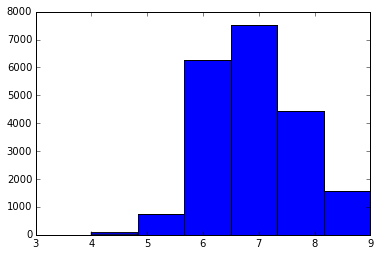
\includegraphics[height=3in]{reliability}
%\end{centering}
%\end{figure}

%While the focus of this paper has been to question the validity of SET as measures of teaching effectiveness, by showing that gender is a stronger predictor of SET scores than student performance, the academic research on SET suggests that reliability may also be an issue. Using the data from Sciences Po, we check for the reliability of students' answers. 







\section{Conclusions}

%Implicit in the use of SET as a Push back on the notion of ``teaching effectiveness.''
%There ought to be \emph{some} interaction between characteristics of the
%instructor and those of the student.
%If ``effectiveness'' is intrinsic to the instructor, ratings in one class shouldn't depend on
%which other classes a student takes.
%Looking at ratings ``per student'' doesn't make sense if you are trying to
%measure some underlying platonic ``effectiveness'' intrinsic to the instructor.
%In particular,  a showing that individual students who give a particular instructor higher ratings
%get higher grades, does not point to ....\todo{fix me}

Teaching effectiveness is a vague notion that even researchers of higher education have a hard time defining. There is a consensus that teaching effectiveness is multidimensional (e.g. \citep{Marsh1997}), and that universities must find incentives to encourage better teaching. The notion of teaching effectiveness implies that instructors have some control over the impact their teaching skills have on student-related outcomes. Measures of teaching effectiveness should therefore only reflect variables that are under the control of instructors. 

In our analysis, we used a robust statistical test to develop the results by \citet{Boring2015} and \citet{MacNell2014}, which suggest that gender biases prevent SET from objectively measuring teaching effectiveness. Our results confirm that an instructor's perceived gender may be more important to students in the way they rate instructors, than student-related outcomes such as an instructor's ability to help student learning. Instructors appear to be rated to a larger extent on a variable that is out of their control (their gender), rather than their ability to positively impact student learning. We further find that the extent and direction of gender biases appear to depend on context. While the French university setting highlights a positive male student bias for male instructors, the experimental US setting suggests a negative female student bias against female instructors.

Instead of measuring teaching effectiveness, SET appear to be a measure of student satisfaction regarding a course \citep{StarkFreishtat2014}. Students may be satisfied or dissatisfied with courses for reasons outside of the control of instructors. Gender may be one of these reasons, due to a given cultural context for example. We do find that the correlation between SET and performance isn't zero:
it can be positive, albeit context dependent and not always statistically significant. While student satisfaction can be considered to be one dimension of teaching effectiveness, the larger point of our analysis is that SET are better measures of student grade expectations and of instructor gender than they are of teaching effectiveness.    

Gender and expected grades are not the only variables unrelated to teaching effectiveness that other studies have shown to be predictors of SET scores. Given the many variables that are likely to bias SET scores and whose weight in SET are likely to change from one learning environment to another, it would be impossible to control for all these variables to make SET a valid measure of teaching effectiveness. Furthermore, the direction of biases appear to be context dependent. 

Among the instructor characteristics alongside gender, race has also been shown to be correlated with SET scores.  In studies conducted in the US, instructors of color appear to suffer from student biases similar to those that female instructors suffer from in our analysis. Minority instructors tend to receive significantly lower SET scores compared to white (male) instructors (e.g. \citet{Merritt2008}).\footnote{French law does not allow for the use of race-related variables in data sets. We were thus unable to test for potential racial biases in SET scores in the context of our French university.} Other instructor-related characteristics likely to be unrelated to teaching effectiveness have been shown to be predictors of SET scores, such as age \citep{Arbuckle2003}, charisma \citep{Shevlin2000} and physical attractiveness (e.g. \citet{Riniolo2006} and \citet{Hamermesh2005}).  

Other factors still unrelated to factors that an instructor can control may be related to SET scores.  Variables related to the teaching environment, class time, class size, mathematical content of the course, etc. may matter. For instance, \citet{Hill2010} show that students' perceptions of classroom environment factors (such as seating characteristics or lighting) have an impact on student ratings of instructors. They find that differences in the physical characteristics of classrooms influence students' overall satisfaction with a course, and have an impact on student evaluations of criteria such as their perceptions of how organized their instructors are.

Hundreds of studies discuss and question the validity of SET as a measure of teaching effectiveness (e.g. for reviews \citet{Pounder2007}). Some studies find results that are similar to ours, with male students expressing biases in favor of male instructors (e.g. \citet{Basow1987}; \citet{Kaschak1978}). Other studies find that the gender and SET is uncorrelated or that the relationship is weak (e.g. \citet{Bennett1982}; \citet{Centra2000}; \citet{Elmore1974}). 
While some studies tend to suggest that SET are not a valid measure of teaching effectiveness {e.g. \citet{Galbraith2012} and \citet{Carrell2010a}), others argue that SET are valid and reliable measures of teaching effectiveness (e.g. \citet{Benton2012} and \citet{Centra1977}). While there is no consensus among academics on the issue of validity, the fact that different studies show such a wide variety of results suggests that validity varies with contexts. This fact, in itself, shows that SET are not universally valid and should be used by universities with great caution.  

In the US, SET have two primary purposes: 
to help instructors improve their teaching and to help the administration make personnel decisions, such as
hiring or promoting instructors. 
We recommend discontinuing the second use of SET, given the strong student biases that 
influence SET, even on ``objective'' items. 
In fact, in France, the French Ministry of Higher Education and Research upheld in 2009 a 1997 decision of the French State Council that public universities can use SET only to help tenured instructors improve their pedagogy, and that the administration may not  use SET in decisions that might affect 
tenured instructors' careers (cf. \citet{Boring2015ofce}). 

Our results suggest that the existence of gender biases in SET is context dependent. 
To test for the external validity of our results, we encourage the replication of our analysis in different settings. The results we find suggest that, in some contexts, female instructors may receive lower than average SET scores, despite being as effective instructors as men, only because of student biases in favor of male instructors. The use of SET therefore unfairly penalizes women, and can have large consequences on their academic careers. Our results more generally emphasize that, at least in some contexts, instructors are being unfairly judged based on variables that are out of their control, potentially leading to negative consequences on their careers in academia. We encourage universities to study potential biases that may occur in their contexts, and to take appropriate measures so as to not penalize instructors for variables that are out of their control.
 

\bibliographystyle{abbrvnat}
\bibliography{SETs}

\end{document}

